\documentclass[12pt]{article}

%%%%%%%%%%%%%%%%%%%%%%%%%%%%%%%%%%%%%%%%%%%%%%%%%%%%%%%%%%%%%%%%%%%%%%%%%%%%%%%%%%%%%%%%%%%
%Package
\usepackage[utf8]{inputenc}  
\usepackage{polski}
\usepackage{fancyvrb}
\usepackage{setspace}
\usepackage[margin=2.5cm]{geometry}
\usepackage{graphicx}
\usepackage{ragged2e}
\usepackage{float}



%%%%%%%%%%%%%%%%%%%%%%%%%%%%%%%%%%%%%%%%%%%%%%%%%%%%%%%%%%%%%%%%%%%%%%%%%%%%%%%%%%%%%%%%%
%Parametry dokumentu
\linespread{1.5}%1.5 odstępu miedzy liniami
\setlength{\parindent}{5pt}
\setlength{\parskip}{1ex plus 0.5ex minus 0.2ex}



%%%%%%%%%%%%%%%%%%%%%%%%%%%%%%%%%%%%%%%%%%%%%%%%%%%%%%%%%%%%%%%%%%%%%%%%%%%%%%%%%%%%%%%%%
\begin{document}
\centering
{\fontsize{20}{20}\selectfont Uniwersytet Przyrodniczy we Wrocławiu}\\
{\fontsize{18}{18}\selectfont Wydział Biologii i Hodowli Zwierząt}\\
{\fontsize{16}{16}\selectfont Kierunek: Bioinformatyka}\\
{\fontsize{16}{16}\selectfont Studia stacjonarne pierwszego stopnia}\\

\vspace{3cm}

{\fontsize{20}{20}\selectfont Dawid Sikorski}\\
{\fontsize{14}{14}\selectfont 110944}\\

\vspace{2.5cm}

\textbf{\fontsize{24}{24}\selectfont Analiza zmienności genetycznej człowieka na podstawie danych z sekwencjonowania nowej generacji}\\
{\fontsize{18}{18}\selectfont Analysis of human genetic variability based on data from next-generation sequencing}\\

\vspace{3cm}

\flushright
{\fontsize{14}{14}\selectfont Praca wykonana pod kierunkiem}\\
{\fontsize{14}{14}\selectfont dr. Tomasz Suchocki}\\
{\fontsize{14}{14}\selectfont Katedra Genetyki}\\

\vspace{2cm}
\centering
{\fontsize{14}{14}\selectfont Wrocław, 2019}\\  

\newpage
 


\flushleft
\vspace{10cm} 
\textbf{\fontsize{14}{14}\selectfont Oświadczenie opiekuna pracy} \\
Oświadczam, że niniejsza praca została przygotowana pod moim kierownictwem i stwierdzam, że spełnia ona warunki do przedstawienia jej w postępowaniu o nadanie tytułu zawodowego.

\vspace{3cm}

Data\hspace{10cm} Podpis opiekuna pracy

\vspace{7cm} 

\textbf{\fontsize{14}{14}\selectfont Oświadczenie autora pracy}\\
Oświadczam, że niniejsza praca dyplomowa została napisana przeze mnie samodzielnie i nie zawiera treści uzyskanych w sposób niezgodny z obowiązującymi przepisami ani też nie była wcześniej przedmiotem procedur związanych z uzyskaniem tytułu zawodowego w wyższej uczelni.

\vspace{3cm}

Data\hspace{10cm} Podpis opiekuna pracy

\newpage

%%%%%%%%%%%%%%%%%%%%%%%%%%%%%%%%%%%%%%%%%%%%%%%%%%%%%%%%%%%%%%%%%%%%%%%%%%%%%%%%%%%%%%%%%
\tableofcontents
%%%%%%%%%%%%%%%%%%%%%%%%%%%%%%%%%%%%%%%%%%%%%%%%%%%%%%%%%%%%%%%%%%%%%%%%%%%%%%%%%%%%%%%%%
\newpage
\justify
\section{Wstęp}\indent

Zmienność genetyczna jest podstawowym mechanizmem ewolucyjnym wszystkich organizmów żywych. Efektem takiej zmienności są różnice w budowie białek, przez co ich funkcji a także czasu i miejscu ich powstania, co może prowadzić do powstania różnic fenotypowych. Wiele z takich cech nie ma jednak znaczenia dla przeżycia organizmu. Rzadko takie zmiany mogą faworyzować dany organizm w środowisku, co dalej prowadzi to rozpowszechnienia cechy a w efekcie do powstania nowego gatunku, który lepiej przystosował się do panujących warunków środowiska. \\
Mimo to większość takich zmian prowadzi do powstania różnych chorób. Badanie zmienności genetycznej człowieka, może dać szansę na poznanie przyczyny ich występowania. Przez badanie różnic w kodzie genetycznym, zauważa się pewne wzory występujących mutacji a pojawiania się pewnych objawów chorobowych. Dzięki takiej wiedzy, przy zastosowaniu technik molekularnego badania genomu, można wykryć mutację która zaszła w DNA i podjąć odpowiednie kroki w celu leczenia objawów danej przypadłości.


\subsection{Rodzaje mutacji i ich konsekwencje}\indent

Poruszane w tej pracy mutacje to:
\begin{itemize}
	\item SNP(ang. Single Nucleotide Polymorphism) - jest to mutacja polegająca na substytucji jednego nukleotyda. SNP stanowią dużą część całkowitej zmienności genetycznej.
	\item Insercja - polega na wstawieniu krótkiego fragmentu nukleotydów lub przynajmniej jednego nukleotydu. 
	\item Delecja - antagonistyczna zmiana do insercji, polegająca na usunięciu conajmniej jednego nukleotydu,
\end{itemize}
Większość zaobserwowanych mutacji nie wywiera żadnego wpływu, ponieważ te negatywne najczęściej są letalne dla organizmu w związku z czym nie występują często. W pracy zwrócono uwagę na 28 różnych konsekwencji mutacji, które zostały kategoryzowane według bazy The Sequence Ontology. 



\subsubsection{Warianty splicingowe} \indent 

\indent Splicing, czyli składanie genu jest ważnym procesem zachodzącym podczas dojrzewania mRNA, poprzez odpowiednie wycinanie intronów, a także eksonów podczas alternatywnego splicingu. Proces ten jest katalizowany przez kompleks białkowo-RNA, który nazywany jest spliceosomem. By intron podlegał wycięciu, musi posiadać dwie silnie konserwatywne sekwencję: GU na końcu 5' oraz AG na końcu 3'. Mutacje tych miejsc mogą prowadzić do poważnych konsekwencji dla organizmu. Kompleks może nie rozpoznać miejsca zachodzenia splicingu, w związku z czym ekson nie zostanie poprawnie złożony, może utracić część łańcucha, przez przedwczesne odczytanie kodonu STOP lub nienaturalnie się wydłużyć. Miejsce splicingowe może zostać przesunięte, powodując zmianę ramki odczytu, delecję lub insercję wielu aminokwasów. 
W przypadku zmiany w sekwencje akceptora(ang. splice acceptor variant) lub donora(ang. splice donor varaint) konsekwencje mutacji są najpoważniejsze, ponieważ dotyczą konserwatywnych sekwencji otaczających ekson. \\
\indent Natomiast wariant regionu splicingowego(ang. splice region variant) dotyczy samych intronów oraz eksonów. Zajście mutacji w takich sekwencjach może skutkować pojawieniem się nowego miejsca splicingowego, przez co część intronu może zostać potraktowana jako ekson, a sam ekson może zostać uznany za intron. Na skutek insercji lub delecji zmieniona może zostać ramka odczytu eksonu, przez co produkt białkowy będzie posiadał inne właściwości. 

\subsubsection{Warianty UTR}
Warianty rejonów nie podlegających translacji 5' i 3' (ang. X5 UTR prime variant and X3 prime UTR variant) - są to regiony, które nie podlegają translacji ale są związane z jego kontrolą. Są one położone terminalnie, po obu stronach regionu podlegającemu translacji, od strony 5' oraz 3'. Zmiany w tych sekwencjach powodują zmiany w strukturach mRNA, jego konformacji i budowy przestrzennej, które biorą udział w kontroli translacji.

\subsubsection{Warianty nie kodujące}

Warianty sekwencji wiążących czynniki transkrypcyjne(ang. TF binding site varaint) \\
W genomie każdego organizmu znajdują się specyficzne sekwencje, do których przyłączają się czynniki transkrypcyjne(ang. TF - transcription factor). Są to tak zwane sekwencje  promotorowe, które warunkują miejsce startu transkrypcji. Mutacje w obrębie tych sekwencji mogą prowadzić to zmniejszenia lub całkowitego zaprzestania ekspresji danego genu, ponieważ czynnik transkrypcyjny nie rozpozna charakterystycznej sekwencji DNA, i w konsekwencji tego nie dojdzie do procesu transkrypcji i dalej translacji.\indent

Ablacja sekwencji wiążących czynniki transkrypcyjne (ang. TFBS ablation) - Jest to rodzaj delecji, która zawiera regiony związane z przyłączaniem się czynników transkrypcyjnych. Podobnie jak w przypadku zmian sekwencji wiążących czynniki transkrypcyjne, usunięcie ich powoduje zmianę ekspresji danego genu.

non coding transcript variant - A sequence variant that changes non-coding exon sequence in a non-coding transcript	 \\
	
non coding transcript exon variant - A transcript variant of a non coding RNA gene	 \\

Warianty regionów regulatorowych (ang. regulatory region variant)  - Większość wariantów związanych z fenotypem człowieka znajduje się w intronach lub regionach między genowych, a więc muszą mieć wpływ na regulacje ekspresji genów. W skład takich sekwencji wchodzą wzmacniacze, a także TATA box, CAAT boxm CCAAT box i inne. Zmiany w tych regionach powodują zmniejszenie lub zwiększenie poziomu ekspresji danego genu.

Warianty dojrzałęgo miRNA(ang. mature miRNA variant) - miRNA lub microRNA jest to mały fragment niekodującego RNA zawierający do 22 nukleotydów.  Jest integralną częścią ekspresji mRNA, wpływając na nią przez obniżanie jej poziomu.  Działają poprzez komplementarne łączenie się z określonymi sekwencjami na mRNA a w efekcie rozerwanie nici mRNA lub jego destabilizacje poprzez skrócenie ogonu poli (A). Zmiany w ci sekwencji mogą powodować hamowanie translacji białek, które docelowo nie miały nimi  być lub dojdzie do nadekspresji jednego z białek.
	
\subsubsection{Warianty między genowe}

Upstream gene variant - A sequence variant located 5' of a gene
	
Downstream gene variant - A sequence variant located 3' of a gene
	
Wariant międzygenowy (ang. intergenetic variant) - Jest to zmiana zachodząca w sekwencji znajdującej się pomiędzy genami i nie pełniąca funkcji regulatorowej. Obecnie ich funkcja jest nieznana.

\subsubsection{Warianty niesynonimiczne}
\indent
\indent Mutacja zmiany sensu (ang. missense variant) - jest to zmiana mogąca prowadzić do zmiany aminokwasu w syntetyzowanym białku. W zależności od substytucji mutacja może nie powodować zmiany funkcji i właściwości posiadanych przez białko (tzw. mutacja konserwatywna), ponieważ nowy aminokwas posiada zbliżone właściwości lub prowadzić do dysfunkcji białka(tzw. mutacja niekonserwatywna)w konsekwencji powstania chorób.


Wariant sekwencji. w którym zmienia się co najmniej jedną zasadę końcowego kodonu niekompletnie opisanego.W kodzie genetycznym występują kodony odpowiadające za terminację translacji: UGA, UAG i UAA. Napotkanie takiej trójki nukleotydowej przez rybosom, jest sygnałem do zakończenia procesu. W przypadku pojawienia się zmian w kodzie jednego z tych kodonów w postaci substytucji, delecji lub insercji, ich funkcje terminacyjne mogą zostać utracone, przeniesione lub za wcześnie zasygnalizują terminacje. Natomiast kodon AUG pełni podwójną funkcje. Jest zarówno sygnałem inicjacji translacji a jednocześnie odczytywany jest przez rybosom jako aminokwas metionina. Wyróżniane są tutaj 4 rodzaje mutacji: \\
Mutacja kodonu STOP, nie zmieniająca jego funkcji (ang. stop retained variant) nie ma wpływu na translacje, ponieważ nie jest ważne który z trójki nukleotydowej zostanie użyty do terminacji procesu. Przykładem takiej zmiany może być mutacja w kodonie UAG przez substytucje 3 nukleotydu czyli guaniny(G) na adeninę(A), w wyniku czego uzyskany kodon UAA dalej pełni funkcję zakończenia translacji. \\
\indent Zmiana powodująca utratę kodonu stop(ang. stop lost) powoduje nienaturalne wydłużenie białka aż do napotkania sygnału terminacji w kodzie kolejnego białka. Konsekwencją takiej mutacji będzie dysfunkcja dwóch białek. \\
\indent Przeciwieństwem do tego jest wariant typy pozyskania kodonu stop(ang. stop gained) w wyniku czego syntetyzowane białko nie osiągnie oczekiwanej długości i właściwości lub powstaną dwa krótkie odcinki polipeptydowe, w przypadku gdy następnym kodenem jest AUG(kodon inicjujący translację), które nie będą posiadały biologicznej funkcji lub będzie ona zaburzona. \\
\indent Na skutek mutacji utraty kodonu start(ang. start lost) pominięty zostanie cały fragment mRNA aż kompleks natrafi na kolejny sygnał startu, który może być składnikiem białka, ponieważ AUG jest rozpoznawane również jako sygnał do syntezy metioniny, w wyniku czego powstanie jedynie fragment docelowego białka o właściwościach bardziej lub mniej podobnych. W przeciwnym przypadku inicjacja rozpocznie się dopiero gdy rybosom odczyta sygnał inicjacji kolejnego produktu transkrypcji. \\
\indent Niekompletny kodon terminacyjny (ang. incomplete terminal codon varaint) - Wariant sekwencji. w którym zmienia się co najmniej jedną zasadę końcowego kodonu niekompletnie opisanego. \\

\subsubsection{Warianty związane z indel'ami}
\indent
\indent Zmiana ramki odczytu (ang. Frameshift variant) - Są to mutacje typu delecja lub insercja powodujące zaburzenia w procesie translacji. W zależności od miejsca zajścia zamiany konsekwencją może być całkowita zmiana łańcucha polipeptydowego lub jego części. Wywierają one bardzo duży wpływ na białko, ponieważ taki produkt najczęściej nie jest w stanie pełnić przeznaczonej funkcji przez zmianę jego budowy lub długości, w konsekwencji organizm nie jest w stanie produkować białka lub jego ilość jest niewystarczająca co ma wpływ na różne szlaki metaboliczne i życie samego organizmu. Jednakże aby do tego doszło zmiana nie może dotyczyć trzech lub wielokrotności tej liczby, gdyż taka zmiana uwzględniając cechę kodu genetycznego jaką jest trójkowość, czyli tworzenie przez trzy nukleotydy kodonu, nie spowoduje zmiany ramki odczytu a jedynie w białku pojawi się nieprawidłowa liczba aminokwasów, przy czym takie białko może zachować swoje właściwości i funkcje. \\

\indent Natomiast warianty typu delecji (ang. inframe deletion) i insercji (ang. inframe insertion) nie zmieniające ramki odczytu są dużo bardziej tolerowane przez organizm. Aby doszło do takiej mutacji, insercja lub delecja musi obejmować krotność liczby 3. W wyniku tego końcowe białko, w zależności od długości indelu (insercji lub delecji), może dalej pełnić swoją funkcję, ponieważ białko może posiadać takie same lub zbliżone właściwości jak niezmutowana wersja.

\subsubsection{Warianty Synonimiczne}
\indent
\indent Wariant intronu (ang. Intron variant) - to zmiana pojawiająca się w sekwencji niekodującej DNA. Takie mutacje nie wywierają lub wywierają wpływ na organizm. Jak powszechnie wiadomo, introny są wykorzystywane w genomie jako sekwencja regulujące transkrypcje, regiony związane ze splicingiem.
	
\indent Wariant synonimiczny (ang. synonymous variant ) - jest to zmiana jednego nukleotydu, który nie powoduje zmiany aminokwasu kodowanego przez triplet. Przykładem takiej mutacji jest zmiana CCC na CCU, w tym przypadku oba kodony odczytywane są jako prolina. 

\subsubsection{Inne}
\begin{itemize}
	\item Wariant sekwencji kodującej (ang. coding sequence variant) - wariant występujący w sekwencji kodującej DNA, powodujących bezpośrednia zmiane na produkt. 
	\item Wariant niekompletnego kodonu terminacyjnego? (ang. incomplete terminal codon variant) - jest to zmiana conajmniej jednego nukleotydu w ostatnim kodonie transkryptu. Nie ma on dużego wpływu na produkt ze względu na to, że proces translacji dobiega końca na tym eksonie, czyli kończy się nić mRNA.
	\item Wariant zmiany białka? (ang. protein altering variant) - jest to zmiana w obrębie sekwencji kodującej białko, która powoduje jego modyfikacje w wyniku czego traci swoje właściwości funkcjonalne lub ich część.
	\item Ablacja transkryptu( ang. transcript ablation) - konsekwencją takiej mutacji jest delecja fragmentu transkryptu, czyli mRNA powstałego na bazie DNA, co ma duży wpływ ze względu na rozległą delecje co prowadzi do niepowstania końcowego produktu lub nie posiada on określonych właściwości przez co jest niefunkcjonalny.
\end{itemize}

\newpage
\subsubsection{Typ wariantu a wpływ na produkt}
\vspace{1cm}
\begin{center}
\begin{tabular}{|l|c|}
Wariant & Wpływ na produkt \\  \hline
X3 prime UTR varaint & Średni\\ 
X5 prime UTR varaint & Średni\\ 
downstream gene varaint & Średni\\ 
frameshift variant & Wysoki\\ 
inframe deletion i inframe insertion & Umiarkowany\\ 
intron variant & Średni\\ 
missense varaint & Umiarkowany\\ 
non coding transcript exon variant & Średni \\ 
non coding transcript variant & Średni\\ 
regulatory region variant & Średni\\ 
splice acceptor varaint & Wysoki\\ 
splice region varaint  & Niski\\ 
splice donor varaint & Wysoki\\ 
start lost & Wysoki\\ 
stop gained & Wysoki\\ 
stop lost & Wysoki\\ 
synosymus varaint & Niski\\ 
TF binding site varaint & Średni\\ 
upstream gene variant & Średni\\ 
coding sequence varaint & Średni\\ 
incomplete terminal codon variant & Niski\\ 
protein altering variant & Umiarkowany\\ 
stop retained variant & Niski\\ 
mature miRNA varian & Średni\\ 
TFBS ablation & Średni\\ 
intergenic variant & Średni\\ 
transcript ablation & Wysoki\\ 
\end{tabular}
\end{center}


\section{Opis genomu człowieka}
\begin{center}
\begin{tabular}{c|c|c}
    Chromosom & Wielkość(w Mb) & Liczba genów  \\  \hline
    1 & 248.96 & 5,109 \\
    2 & 242.19 & 3,871 \\
    3 & 198.3 & 2,990 \\
    4 & 190.22 & 2,441 \\
    5 & 181.54 & 2,592 \\
    6 & 170.81 & 3,005 \\
    7 & 159.35 & 2,792 \\
    8 & 145.14 & 2,165 \\
    9 & 138.4 & 2,270 \\
    10 & 133.8 & 2,179 \\
    11 & 135.09	& 2,924 \\
    12 & 133.28 & 2,526 \\
    13 & 114.36 & 1,385 \\
    14 & 107.04	& 2,065 \\
    15 & 101.99 & 1,824 \\
    16 & 90.34 & 1,938 \\
    17 & 83.26 & 2,450 \\
    18 & 80.37 & 984 \\
    19 & 58.62 & 2,499 \\
    20 & 64.44 & 1,358 \\
    21 & 46.71 & 777 \\
    22 & 50.82 & 1,189 \\
\end{tabular}
\end{center}

\section{Cel pracy}\indent

Celem pracy jest analiza zmienności genetycznej człowieka. Praca omawia zależności pomiędzy ilością wariantów a ich lokalizacją w kariotypie oraz konsekwencją mutacji, a także rozważania na temat samych konsekwencji mutacji. Przedstawione zostaną wariantów, jakie wywierają zmiany w DNA oraz dlaczego niektóre są akceptowane przez organizm a inne powodują jego śmierć. Przedstawione zostaną informacje o liczebności wariantów, ich rozłożeniu na chromosomach i frekwencji pojawiania się. 








\section{Materiały i metodyka}

\subsection{Użyte oprogramowanie?}\indent
W pracy użyto wymienione programy i aplikacje:
\begin{itemize}
    \item Python w wersji 3.7.2
    opis ile i jakie skrypty powstały?
    \item RStudio w wersji 3.5.1
    co robiłem i jakich paczek uzyłem?
    \item Linux i bash
    \item Bedtools w wersji 2.28.0

\end{itemize}
\subsection{Baza danych}

\indent Niniejsza praca oparta jest na zestawie danych pochodzących z gnomAD (genome aggregation database). Jest to baza danych opracowana przez międzynarodową koalicję badaczy, w celu agregowania i ujednolicenia danych dotyczących szerokiej gamy projektów sekwencjonowania genomu oraz udostępniania tych danych dla społeczności naukowej. \\

Baza danych obejmuje 125 748 sekwencji egzomowych oraz 15 708 sekwencji całego genomu od niepowiązanych osobników zsekwencjonowanych w ramach różnych badań genetycznych specyficznych dla choroby i populacji.

\indent
Użyty zestaw danych zawiera informacje o wariancjach z 22 chromosomów autosomalnych, oraz zawiera 119794797 indywidualnych rekordów. Dostarczają one informacji o miejscu wystąpienia danej mutacji, czyli chromosomie i jego pozycji w nim, porównuje zmieniony fragment z próbą kontrolną, a także dostarcza informacji o jego frekwencji i ilości z jaką występował podczas tworzenia bazy. 

\subsection{Opis formatu VCF}\
indent Variant Call Format(VCF) jest to unikalny format plików tekstowych używany w bioinformatyce do przechowywania danych genomu dotyczących mutacji. Format został opracowany wraz z rozpoczęciem projektów sekwencjonowania genomów na dużą skalę, takich jak 1000 Genomes Project. 

Nagłówek rozpoczyna plik i opisuje jego zawartość. Linie nagłówka są oznaczone jako {\#}. Specjalne słowa kluczowe w nagłówku są oznaczone {\# \#}. Zawierają one informacje o pochodzeniu pliku, gatunku oraz objaśniają użyte w nim skróty.
\begin{figure}[!htbp] 
  \centering
    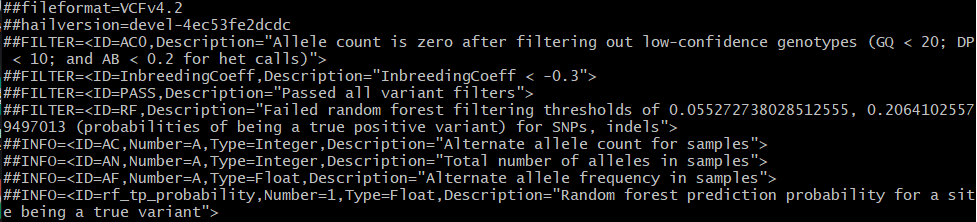
\includegraphics[scale=0.66]{VCF/VCF_header.PNG}
    \caption{Fragment nagłówka z użytego zestawu danych}
\end{figure}

\begin{center}
\begin{tabular}{|l|l|l|}
 \hline
 &Nazwa&Krótki opis.\\  \hline
1&Chrom&Numer chromosomu, na którym znajduje się dany wariant. \\ \hline
2&POS&Pozycja zmiany w sekwencji. \\  \hline
3&ID&Identyfikator zmiany.  \\  \hline
4&REF&Allel referencyjny, czyli allel według genomu referencyjnego.  \\  \hline
5&ALT&Allel alternatywny, czyli allel jaki pojawił się u osobnika o danym wariancie.  \\  \hline
6&QUAL&Prawdopodobieństwo, że polimorfizm Ref/ALT występuje w tym miejscu w skali phred   \\  \hline
7&FILTER&Zawiera informacje na temat których filtrów dany rekord nie przeszedł. \\  \hline
8&INFO&Lista zawierająca zastawy klucz-wartość, opisująca wariant. \\  \hline
\end{tabular}\\
\end{center} 

\vspace{1cm}

Pole info zawiera szczegółowe informacje rekordu.
Wykorzystane w pracy kategorie to:
AC=3, liczba alleli w genotypach
AN=2654, całkowita liczba alleli w użytych genotypach
AF=1.13037e-03, częstość występowania danego allelu
vep, zawierający szczegółowe informacje na temat wariantu takie jak: \\
Typ wariantu, wpływ na produkt, identyfikatory dla biologicznych baz danych(NCBI oraz ENSEMBL) i wiele innych, które nie zostały użyte na potrzeby pracy.

\begin{figure}[H]
  \centering
    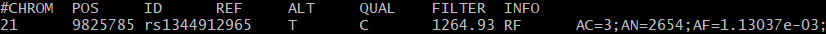
\includegraphics[scale=0.78]{VCF/VCF_1stline.PNG}
    \caption{Fragment pliku przedstawiający dane}
\end{figure}

\subsection{Przetwarzanie pliku VCF}\indent

Z racji dużego rozmiaru pliku oraz zawartości niepotrzebnych informacji, plik ten musiał zostać odpowiednio przygotowany zanim zostanie użyty do przeprowadzenia analizy. \\ 
W tym celu został stworzony krótki skrypt w Pythonie, którego zadaniem była ekstrakcja kluczowych dla analizy danych.


Kod skryptu użytego do wydobycia danych \\
potrzebne?
\begin{verbatim}
with open
('/home/dawid/Pulpit/Variant_analysis_data/gnomad.exomes.r2.1.sites.chr21.vcf' ,'r')
as input_file,
open('/home/dawid/Pulpit/Variant_analysis_data/data_1.txt','w')
as output_file:
    for line in input_file:
        if line[0][0] == '#':
            continue
        line = line.split('\t')
        temp = [line[i] for i in [0,1,3,4]]
        info = line[7].split(';')
        info[0] = info[0][len('AC='):]
        info[1] = info[1][len('AN='):]
        info[2] = info[2][len('AF='):]
        vep = info[-1].split(',')
        if line[6] == 'PASS':
            for ele in vep:
                vep_info = ele.strip().split('|')
                vep_info = [vep_info[i] for i in [1,2,3,4,5,6,22]]
                output_file.write('\t'.join(temp+info[0:3]+vep_info)+'\n')    

\end{verbatim}


\section{Wyniki}
\begin{figure}[H]
    \includegraphics[width=1\textwidth]{hist_all_variants.png}
    \caption{Histogram przedstawiający stosunek ogólnej liczby wariantów}
\end{figure}
Dominującymi kategoriami są intergenetic variant, intron variant oraz non synonymous variant. Duże liczebności dwóch pierwszych kategoria wynikają z miejsca ich występowania. Regiony międzygenowe jak i introny ze względu na brak niesienia informacji genetycznej, są dość zmienne i niekonserwatywne. Zmiany w ich obrębie przeważnie nie objawiają się fenotypowo, chyba że dotyczą regionów regulatorowych zmieniając poziom ekspresji. Natomiast mutacje niesynonimiczne, czyli zmieniające aminokwas występujący w białku, w większości przypadków nie wpływa na produkt. Zmiana do kilku aminokwasów może nie zmienić zbytnio właściwości białka dzięki czemu będzie ono dalej funkcjonalne. Najmniej wariantów obserwuję się dla kategorii frameshift, inframe indel oraz other, które zawierają kategorie: coding sequence variant, transcript ablation oraz protein altering variant. Zmiany tego typu zazwyczaj niosą poważne konsekwencje w związku z czym nie są tolerowane przez organizm i mogą prowadzić do chorób lub śmierci. 
\begin{figure}[H]
    \includegraphics[width=1\textwidth]{hist_prot_variants.png}
    \caption{Histogram przedstawiający stosunek ogólnej liczby wariantów w przypadku wariantów związanych z białkami}
\end{figure}

Natomiast w przypadku wariantów związanych z białkami dominującymi kategoriami są missense variant oraz synonymous variant. Warianty missensowne często mają mały wpływ na białko, przez to mutacje tego typu są akceptowane przez organizm. Dochodzi do tego gdy aminokwas zostaję zastąpiony innym, ale o zbliżonych właściwościach, dzięki czemu białko zachowuje swoją funkcje. Rzadziej zostaje podmieniony na taki, który powoduję zmianę funkcji białka. Takie mutacje mogą prowadzić do zaburzeń lub śmierci. Warianty synonimiczne czyli ciche nie powodują zmiany w kodowanym aminokwasie i nie ma wpływu na funkcjonowanie organizmu. 
\subsection{Warianty dotyczące białek}

\subsubsection{Wykresy dotyczące liczebności wariantów}

\begin{figure}[H]
    \includegraphics[width=1\textwidth]{Warianty_bialkowe/bar_plot_varaint_count_prot.png}
    \caption{Wykres przedstawiający ilość wariantu na danym chromosomie}
\end{figure}
\indent
\indent Analizując powyższy wykres stwierdzono, że największa ilość wariantów zlokalizowana jest na chromosomie 1, co wynika z faktu że jest to największy chromosom i posiada największą ilość genów. Natomiast chromosom 2 i 19 posiada zbliżoną liczbę wariantów, pomimo tego że chromosom 2 posiada 3,871 genów i wielkość równą 242.19 a chromosom 19 - 2,499 genów i wielkość równa 58.62. Wynika z tego, że chromosom 19 cechuję się stosunkowo małą konserwatywnością. Niewielka liczba wariantów na chromosomie 13 może wynikać z małej liczby genów (1,385), dla porównania podobną liczbę posiada chromosom 20 (1,358), biorąc pod uwagę jego wielkość (114.36 Mb) można wnioskować o dużej liczbie i wielkości regionów niekodujących. 

\begin{figure}[H]
    \includegraphics[width=1\textwidth]{Warianty_bialkowe/stacked_bar_plot_varaint_count.png}
    \caption{Wykres przedstawiający procentowy udział ilości wariantów na danym chromosomie}
\end{figure}
\indent
\indent Rozłożenie wariantów na poszczególnych chromosomach jest stosunkowo równe. Największy odsetek stanowią: 
\begin{itemize}
    \item Warianty missensowne (ang. missense\_variant)
    \item Warianty synonimiczne (ang. synonymous\_variant)
    \item Warianty splicingowe (ang. splicing)
\end{itemize}
Analizując wykres, stwierdzono ze wyżej wymienione warianty znajdują się pod najmniejszą presją ewolucyjną i powodują największą zmienność fenotypową. Pozostałe warianty pojawiają się bardzo rzadko. Jest to spowodowane ich wpływem na organizm, który musi nieść ze sobą negatywny efekt lub być letalnym dla organizmu. 
\begin{figure}[H]
    \includegraphics[width=1\textwidth]{Warianty_bialkowe/bar_plot_variant_count_prot_other.png}
    \caption{Wykres przedstawiający warianty zawarte w kategorii 'Other'}
\end{figure}



\subsubsection{Wykresy dotyczące frekwencji wariantów}
\begin{figure}[H]
    \includegraphics[width=1\textwidth]{Warianty_bialkowe/bar_plot_AF_mean_prot.png}
    \caption{Wykres przedstawiający frekwencję wariantów na danym chromosomie}
\end{figure}
\begin{figure}[H]
    \includegraphics[width=1\textwidth]{Warianty_bialkowe/bar_plot_AF_mean_prot_other.png}
    \caption{Wykres przedstawiający frekwencje wariantó w kategori 'Other'}
\end{figure}
\begin{figure}[H]
    \includegraphics[width=1\textwidth]{Warianty_bialkowe/stacked_bar_plot_variant_count_prot_other.png}
    \caption{Wykres przedstawiający procentowy udział frekwencji w kategorii 'Other'}
\end{figure}
wykres2 \\

\subsection{Wszystkie warianty genomu}
wykres1 \\
wykres2 \\

\newpage
\section{Bibliografia}

\begin{verbatim}
https://en.wikipedia.org/wiki/Variant_Call_Format
https://www.ensembl.org/info/genome/variation/prediction/predicted_data.html
https://www.ncbi.nlm.nih.gov/pmc/articles/PMC5635616/
https://www.ncbi.nlm.nih.gov/pmc/articles/PMC4445073/
https://www.ncbi.nlm.nih.gov/pmc/articles/PMC4797991/
(How do microRNAs regulate gene expression?
Ian G. Cannell1, Yi Wen Kong1 and Martin Bushell2
School of Pharmacy, Centre for Biomolecular Sciences, University of Nottingham, University Park, Nottingham NG7 2RD, U.K)https://www.ncbi.nlm.nih.gov/pubmed/19021530
https://onlinelibrary.wiley.com/doi/abs/10.1002/wrna.1451
https://www.ncbi.nlm.nih.gov/genome?LinkName=assembly_genome&from_uid=1493941
\end{verbatim}

\end{document}
